\documentclass[11pt,a4paper]{report}
\PassOptionsToPackage{table}{xcolor}
\usepackage[T1]{fontenc}
\usepackage[margin=2.3cm]{geometry}
\usepackage{graphicx,xcolor,booktabs,longtable,array,enumitem}
\usepackage{fancyhdr,titlesec,hyperref}
\usepackage{tikz}
\usetikzlibrary{positioning,shapes.geometric,arrows.meta,calc,fit,backgrounds,decorations.pathreplacing}
\usepackage[most]{tcolorbox}
\usepackage{listings}

% ---------------- palette ----------------
\definecolor{pblue}{HTML}{2563EB}
\definecolor{pdark}{HTML}{14181F}
\definecolor{pslate}{HTML}{334155}
\definecolor{danger}{HTML}{DC2626}
\definecolor{warn}{HTML}{D97706}
\definecolor{tip}{HTML}{16A34A}
\definecolor{note}{HTML}{0891B2}
\definecolor{codebg}{HTML}{F5F7FA}
\definecolor{kw}{HTML}{2563EB}
\definecolor{cmt}{HTML}{6B7280}
\definecolor{str}{HTML}{16A34A}
\definecolor{num}{HTML}{9333EA}
\definecolor{rowalt}{HTML}{EEF3FB}

\hypersetup{colorlinks=true,linkcolor=pblue,urlcolor=pblue,citecolor=pblue}
\pagestyle{fancy}\fancyhf{}
\rhead{\textcolor{pslate}{\small PROACT Manual}}\lhead{\textcolor{pslate}{\small\leftmark}}
\rfoot{\thepage}\renewcommand{\headrulewidth}{0.4pt}
\titleformat{\chapter}[display]{\bfseries\color{pblue}}{\Large CHAPTER \thechapter}{4pt}{\Huge}
\titlespacing*{\chapter}{0pt}{-10pt}{20pt}

\newcommand{\code}[1]{{\ttfamily\small #1}}
\graphicspath{{../images/}}

% ---------------- callout boxes ----------------
\newtcolorbox{danger}{colback=note!6,colframe=note,coltitle=white,
  fonttitle=\bfseries,title=SOFTWARE RULE,boxrule=1pt,arc=3pt,left=6pt,right=6pt,breakable}
\newtcolorbox{warnbox}{colback=warn!7,colframe=warn,coltitle=white,
  fonttitle=\bfseries,title=WARNING,boxrule=1pt,arc=3pt,left=6pt,right=6pt,breakable}
\newtcolorbox{tipbox}{colback=tip!7,colframe=tip,coltitle=white,
  fonttitle=\bfseries,title=TIP,boxrule=1pt,arc=3pt,left=6pt,right=6pt,breakable}
\newtcolorbox{notebox}{colback=note!7,colframe=note,coltitle=white,
  fonttitle=\bfseries,title=NOTE,boxrule=1pt,arc=3pt,left=6pt,right=6pt,breakable}
\newtcolorbox{factbox}{colback=pblue!6,colframe=pblue,coltitle=white,
  fonttitle=\bfseries,title=HARDWARE FACT (frozen),boxrule=1pt,arc=3pt,left=6pt,right=6pt,breakable}

% ---------------- code listings ----------------
\lstdefinestyle{base}{backgroundcolor=\color{codebg},basicstyle=\ttfamily\footnotesize,
  keywordstyle=\color{kw}\bfseries,commentstyle=\color{cmt}\itshape,stringstyle=\color{str},
  numberstyle=\tiny\color{cmt},numbers=left,numbersep=7pt,frame=leftline,framerule=2pt,
  rulecolor=\color{pblue},breaklines=true,showstringspaces=false,tabsize=2,columns=fullflexible,
  literate={0x}{{\color{num}0x}}2 }
\lstdefinestyle{c}{style=base,language=C,morekeywords={uint32_t,uint8_t,uintptr_t,int32_t}}
\lstdefinestyle{py}{style=base,language=Python}
\lstdefinestyle{sh}{style=base,language=bash,keywordstyle=\color{pblue}\bfseries}
\lstset{style=base}

\begin{document}

% ================= TITLE =================
\begin{titlepage}\centering
\begin{tikzpicture}[remember picture,overlay]
  \fill[pdark] (current page.north west) rectangle ([yshift=-6.5cm]current page.north east);
\end{tikzpicture}
\vspace*{1.2cm}
{\color{white}\Huge\bfseries PROACT}\\[6pt]
{\color{white!85}\Large The Complete Manual}\\[4pt]
{\color{pblue!40}\large Software $\cdot$ Firmware $\cdot$ Python $\cdot$ GUI $\cdot$ ChipWhisperer}\\[5cm]
{\Large\bfseries A lightweight-crypto RISC-V SoC (ASIC + FPGA)}\\[3pt]
{\large Version 1.1 \quad--\quad addresses, hardware, C library, host library, GUI and trace capture}\\[1.4cm]
\begin{danger}
The PROACT chip is \textbf{fabricated and frozen}: the RTL is the read-only,
authoritative reference and the software follows it exactly. PROACT is a compact,
area-optimized side-channel research SoC; its lean peripherals expect a few simple
software access conventions, which the drivers in this repository already implement.
Chapter 2 documents those conventions so the behavior is fully understood.
\end{danger}
\vfill
{\small Generated from the maintained sources in this repository
(\code{config/hardware.json}, the firmware/host code, and the Markdown docs).}
\end{titlepage}

\tableofcontents

% ================= CH1 OVERVIEW =================
\chapter{Introduction and System Overview}
PROACT is a dual-core RISC-V system-on-chip designed for \emph{side-channel
research}: measuring the power consumption of cryptographic operations to study
their resistance to attacks such as CPA, TVLA and SNR. It was fabricated on the
GlobalFoundries 22FDX process (tape-out November 2025) and the same design also
runs on FPGA (ChipWhisperer CW305 / PYNQ-Z2).

\section{System components}
Two Ibex RISC-V cores share a bus:
\begin{itemize}[leftmargin=1.4em]
\item the \textbf{controller} --- communicates with the host PC (UART commands, SPI code
loading) and drives the crypto cores and the scope trigger;
\item the \textbf{Sw-RV target} --- a second core that runs \emph{software} AES,
so hardware and software crypto can be compared on the same silicon.
\end{itemize}
Four hardware crypto cores are attached to the bus: \textbf{AES1}, \textbf{AES2}
(AES-128, encrypt + decrypt) and \textbf{ASCON}, \textbf{Xoodyak} (authenticated
encryption; the cores implement the encryption datapath and decrypt runs on the
host, see Ch.~6). Supporting peripherals: a UART, an SPI code loader, a timer
that measures the trigger window, and an LFSR RNG.

% Drop-in for the original colour block diagram; if the source PNG exists at
% docs/images/architecture.png it is used instead of the TikZ drawing.
\begin{center}
\IfFileExists{../images/architecture.png}{%
  
\includegraphics[width=0.9\textwidth]{architecture.png}%
}{%
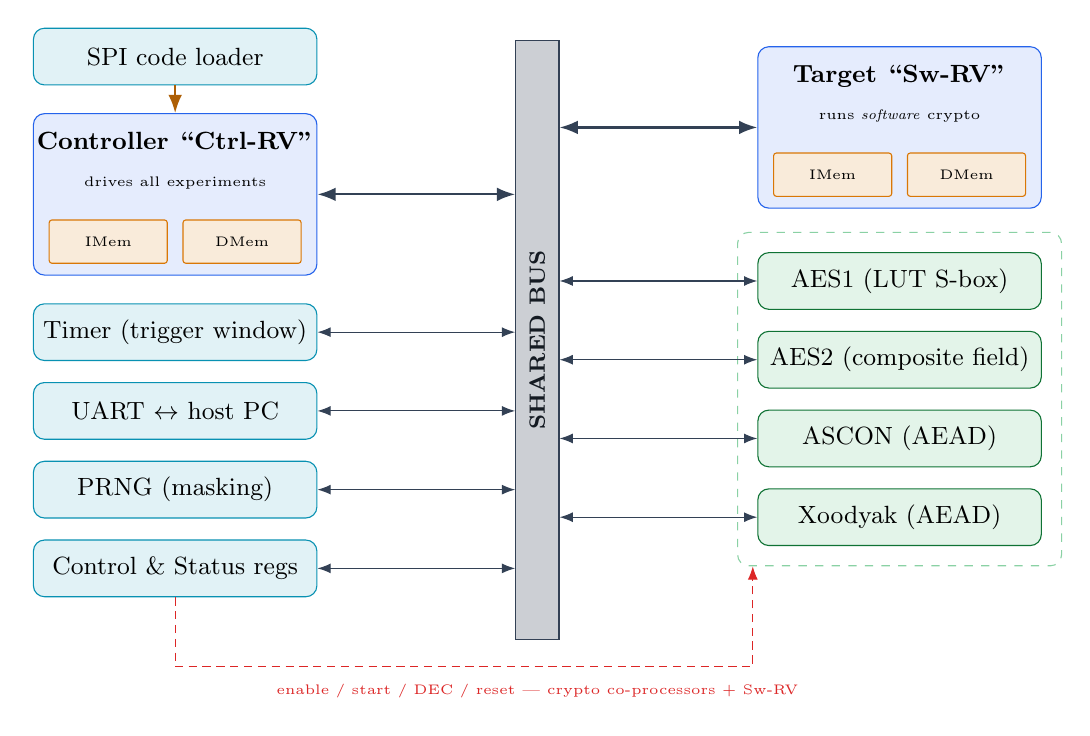
\begin{tikzpicture}[font=\small,>=Latex,
  cpu/.style={draw=pblue,fill=pblue!12,rounded corners,minimum width=3.6cm,minimum height=2.05cm},
  cry/.style={draw=tip!70!black,fill=tip!12,rounded corners,minimum width=3.6cm,minimum height=0.72cm,align=center},
  per/.style={draw=note,fill=note!12,rounded corners,minimum width=3.6cm,minimum height=0.72cm,align=center},
  mem/.style={draw=warn,fill=warn!15,rounded corners=1pt,minimum width=1.5cm,minimum height=0.55cm,align=center,font=\tiny},
  bus/.style={draw=pslate,fill=pslate!25,minimum width=0.55cm,minimum height=7.6cm,inner sep=0pt}]
  % the shared bus, vertical spine in the middle
  \node[bus] (bus) at (0,-0.2) {};
  \node[rotate=90,font=\footnotesize\bfseries,text=pslate!40!black] at (bus.center) {SHARED BUS};

  % ---------------- left: controller side ----------------
  \node[per] (spi) at (-4.6,3.4) {SPI code loader};
  \node[cpu] (ctrl) at (-4.6,1.65) {};
  \node[anchor=north,font=\small\bfseries] at ([yshift=-1.2mm]ctrl.north) {Controller ``Ctrl-RV''};
  \node[anchor=north,font=\tiny] at ([yshift=-6.8mm]ctrl.north) {drives all experiments};
  \node[mem,anchor=south west] at ([xshift=2mm,yshift=1.5mm]ctrl.south west) {IMem};
  \node[mem,anchor=south east] at ([xshift=-2mm,yshift=1.5mm]ctrl.south east) {DMem};
  \node[per] (timer) at (-4.6,-0.1) {Timer (trigger window)};
  \node[per] (uart) at (-4.6,-1.1) {UART $\leftrightarrow$ host PC};
  \node[per] (prng) at (-4.6,-2.1) {PRNG (masking)};
  \node[per] (cs) at (-4.6,-3.1) {Control \& Status regs};
  \draw[->,thick,warn!80!black] (spi) -- (ctrl);
  \draw[<->,thick,pslate] (ctrl.east) -- (ctrl.east -| bus.west);
  \foreach \n in {timer,uart,prng,cs} \draw[<->,pslate] (\n.east) -- (\n.east -| bus.west);

  % ---------------- right: target side ----------------
  \node[cpu] (tgt) at (4.6,2.5) {};
  \node[anchor=north,font=\small\bfseries] at ([yshift=-1.2mm]tgt.north) {Target ``Sw-RV''};
  \node[anchor=north,font=\tiny] at ([yshift=-6.8mm]tgt.north) {runs \emph{software} crypto};
  \node[mem,anchor=south west] at ([xshift=2mm,yshift=1.5mm]tgt.south west) {IMem};
  \node[mem,anchor=south east] at ([xshift=-2mm,yshift=1.5mm]tgt.south east) {DMem};
  \node[cry] (a1) at (4.6,0.55) {AES1 (LUT S-box)};
  \node[cry] (a2) at (4.6,-0.45) {AES2 (composite field)};
  \node[cry] (as) at (4.6,-1.45) {ASCON (AEAD)};
  \node[cry] (xo) at (4.6,-2.45) {Xoodyak (AEAD)};
  \begin{scope}[on background layer]
    \node[draw=tip!50,dashed,rounded corners,fit=(a1)(xo),inner sep=2.5mm] (cryptogrp) {};
  \end{scope}
  \draw[<->,thick,pslate] (tgt.west) -- (tgt.west -| bus.east);
  \foreach \n in {a1,a2,as,xo} \draw[<->,pslate] (\n.west) -- (\n.west -| bus.east);

  % control fan-out: the C&S register enables/starts/resets the cores + Sw-RV
  \draw[densely dashed,->,danger] (cs.south) |- (0,-4.35) -| ([xshift=2mm]cryptogrp.south west);
  \node[font=\tiny,text=danger,anchor=north] at (0,-4.45)
    {enable / start / DEC / reset --- crypto co-processors + Sw-RV};
\end{tikzpicture}}
\end{center}

\begin{factbox}
For \textbf{software}, the ASIC and the FPGA are the \emph{same machine}: the
address map is byte-for-byte identical. They differ only in memories, register
file, debug pins and clocking --- none of which the software can see.
\end{factbox}

\section{Software architecture}
One JSON file, \code{config/hardware.json}, is the single source of truth for
every address and register bit. \code{scripts/gen\_hardware.py} generates the
C header (\code{proact\_regs.h}) and the Python module (\code{regs.py}) from it,
so the firmware, the host tools and this manual cannot disagree. One Python
package, \code{proact\_host}, is shared by the command-line tool, the GUI and
user scripts.

% ================= CH2 GOLDEN RULES =================
\chapter{Design Characteristics and Software Rules}
PROACT is a compact, area-optimized side-channel research SoC. To keep the
silicon small and the power signatures clean, the bus and peripherals are
deliberately minimal --- for example the shared bus has no access watchdog: each
peripheral answers an access when its data is ready. This is an efficient,
common bare-metal design; it simply means the software follows a short list of
access conventions. \textbf{The drivers and the \code{proact\_host} library
already implement every rule below}, so in normal use they require no direct attention.
This chapter documents the behavior so it is fully understood and so anyone
extending the firmware keeps the same conventions.

\begin{center}
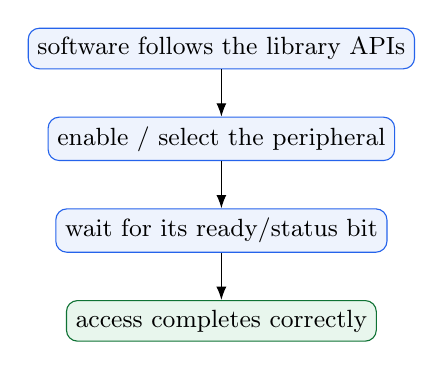
\begin{tikzpicture}[font=\small,node distance=6mm,
  b/.style={draw=pblue,rounded corners,fill=pblue!8,minimum width=3.8cm,align=center},
  g/.style={draw=tip!70!black,fill=tip!10,rounded corners,align=center,minimum width=3.8cm}]
  \node[b] (acc) {software follows the library APIs};
  \node[b,below=of acc] (en) {enable / select the peripheral};
  \node[b,below=of en] (wait) {wait for its ready/status bit};
  \node[g,below=of wait] (ok) {access completes correctly};
  \draw[-Latex] (acc)--(en); \draw[-Latex] (en)--(wait); \draw[-Latex] (wait)--(ok);
\end{tikzpicture}
\end{center}

\begin{danger}
The access conventions (all handled by the drivers):
\begin{enumerate}[leftmargin=1.4em,nosep]
\item \code{0x10007000} (\code{Co\_re}) is a reserved expansion slot with no core
attached in this revision --- do not access it.
\item Set a crypto core's \code{ENABLE} bit before accessing its registers; run
one core at a time (clean power-gating keeps unused cores quiet).
\item UART writes use offsets \code{0x00} (data) and \code{0x04} (baud) --- use
\code{putchar()} / \code{uart\_set\_baud\_divisor()}.
\item UART receive uses the status handshake: poll status-register bit 0
(\code{STAT\_UART\_RVALID} = ``RX FIFO not empty''), then read the byte.
\code{uart\_getchar()} does this.
\end{enumerate}
\end{danger}

\begin{notebox}
\textbf{Note --- UART TX FIFO depth.} The transmit FIFO holds 512 bytes.
Output produced faster than the serial line drains it fills the FIFO, so the
firmware paces \code{putchar()} to stay within the line rate (scale the pacing if
the baud rate is lowered). This keeps verbose logging lossless.
\end{notebox}

\begin{factbox}
\textbf{Global trigger = control bit 30} (\code{0x40000000}), confirmed by the
hardware design team. The control register carries 31 defined bits, so the trigger
(the register's top defined bit) is bit 30. The \emph{status} register is a full
32-bit register, and status bit 0 is the UART ``RX not-empty'' flag while status
bit 31 is the Sw-RV ``target done'' / Sw-RV trigger source.
\end{factbox}

The full set with the software rule for each is in \code{docs/hardware\_hazards.md}
(rules R1--R10; R10 is the AEAD rule --- ASCON/Xoodyak decrypt runs on the host,
see Ch.~6).

% ================= CH3 INSTALL =================
\chapter{Installation and Setup}
\section{Prerequisites}
\begin{center}\rowcolors{2}{rowalt}{white}
\begin{tabular}{p{5cm}p{9cm}}
\toprule
\textbf{Purpose} & \textbf{Tool} \\ \midrule
Build firmware & \code{riscv32-unknown-elf-gcc} + \code{srec\_cat} \\
Host control / capture & Python $\geq$ 3.9 (\code{requirements.txt}) \\
USB bridges & MCP2200 (UART) + MCP2210 (SPI), via \code{hidapi} \\
Capture (optional) & ChipWhisperer 6 (CW305 + Husky) \\
RTL simulation (optional) & Icarus Verilog $\geq$ 11 \\
PDF manual (optional) & \code{pdflatex} (TeX Live) \\
\bottomrule
\end{tabular}\end{center}

\section{Install the host tools}
The ``host tools'' are the PC-side Python package
(\code{proact\_host}) plus the CLI and GUI that run on the host PC
and communicate with the PROACT board over USB. Nothing here runs \emph{on} the
chip --- these tools program the chip, send it commands, read results,
and capture power traces. Installing them lets the CLI, the GUI and user
scripts share one tested library instead of each re-implementing the serial
protocol. The recommended install is one command, followed by \emph{always}
launching through the wrapper scripts:
\begin{lstlisting}[style=sh]
bash tools/setup_env.sh   # one-time: builds a dedicated venv at ~/.proact-venv
./run_cli.sh info         # the CLI -- prints the address map, no board needed
./run_gui.sh              # the GUI
\end{lstlisting}
The wrappers pick the right interpreter automatically. This avoids the common
pitfall where a bare \code{python3} (e.g.\ a pyenv shim) is a \emph{different}
Python that is missing \code{PyQt6}/\code{hid}/\code{mcp2210}/%
\code{chipwhisperer}. For a manually managed environment, install
\code{requirements.txt} plus \code{pip install -e Software/Python[all]} (adds
the \code{proact} CLI entry point).
\begin{warnbox}
\textbf{Never run the tools with \code{sudo}.} Running as root \emph{breaks} the
ChipWhisperer install (it lives under the invoking user's \code{\~{}/.local}).
Device access comes from the udev rules instead --- see the USB permissions
section below.
\end{warnbox}

\section{Build the firmware}
The two RISC-V cores run C programs compiled in this step: the
\emph{controller} firmware (the command server the host communicates with) and the
\emph{target} firmware (software AES on the Sw-RV core). \code{make} cross-compiles
them and produces \code{.vmem} images that are loaded into the chip's memories.
\begin{lstlisting}[style=sh]
make -C Software/Controller RISCV=riscv32-unknown-elf-   # -> main.vmem (one image)
make -C Software/SW_RV      RISCV=riscv32-unknown-elf-    # -> sw_rv_*.vmem (two)
\end{lstlisting}
\begin{tipbox}
No local paths are hard-coded. The toolchain prefix is the \code{RISCV} make
variable; override it on the command line. Bench constants (MCP serials, input
clock, reset-pin polarity) all live in \code{proact\_host/config.py}.
\end{tipbox}

\section{USB permissions (Linux) --- avoiding \code{sudo}}
The MCP2200 (UART), MCP2210 (SPI) and the ChipWhisperer are USB devices that by
default only root can open. Fix this \emph{once} with the provided installer ---
do \textbf{not} work around it with \code{sudo}:
\begin{lstlisting}[style=sh]
sudo bash tools/install_udev.sh   # installs udev/60-proact.rules (MCP + all
                                  # NewAE devices) and adds you to `dialout`
# then UNPLUG and REPLUG the USB devices (log out/in for the group change)
\end{lstlisting}
After that, everything runs under the normal user account via \code{./run\_cli.sh} /
\code{./run\_gui.sh}.

% ================= CH4 MEMORY MAP =================
\chapter{Memory and Address Map}
Every value is generated from \code{config/hardware.json} and cross-checked
against the frozen RTL (34 automated checks pass, \code{tools/verify\_regs\_vs\_rtl.py}).

\begin{center}
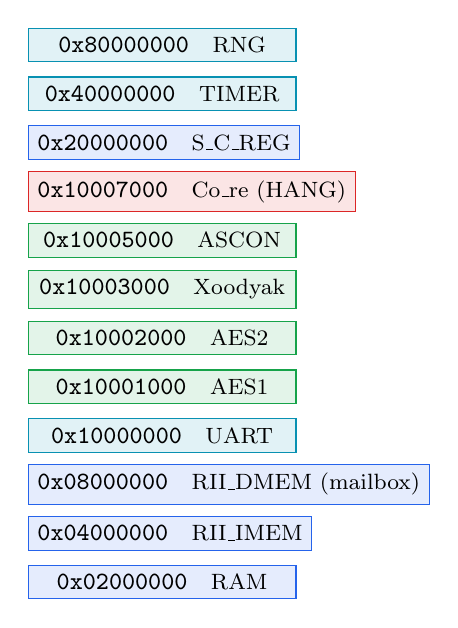
\begin{tikzpicture}[font=\footnotesize,y=0.62cm,
  m/.style={draw,minimum width=3.4cm,anchor=west,align=left}]
  \foreach \y/\a/\n/\c in {
    11/0x80000000/RNG/note, 10/0x40000000/TIMER/note, 9/0x20000000/S\_C\_REG/pblue,
    8/0x10007000/Co\_re (HANG)/danger, 7/0x10005000/ASCON/tip, 6/0x10003000/Xoodyak/tip,
    5/0x10002000/AES2/tip, 4/0x10001000/AES1/tip, 3/0x10000000/UART/note,
    2/0x08000000/RII\_DMEM (mailbox)/pblue, 1/0x04000000/RII\_IMEM/pblue, 0/0x02000000/RAM/pblue}
    {\node[m,fill=\c!12,draw=\c] at (0,\y) {\code{\a}\quad \n};}
\end{tikzpicture}
\end{center}

\begin{center}\rowcolors{2}{rowalt}{white}
\begin{longtable}{lll p{6.4cm}}
\toprule
Device & Base & Region & Notes \\ \midrule\endhead
RAM & \code{0x02000000} & 32\,MB & controller data RAM (128\,KB phys) \\
RII\_IMEM & \code{0x04000000} & 32\,MB & Sw-RV instruction memory write port \\
RII\_DMEM & \code{0x08000000} & 128\,MB & Sw-RV data mem; controller$\leftrightarrow$target mailbox \\
S\_C\_REG & \code{0x20000000} & 1\,KB & WRITE = control, READ = status (same addr) \\
UART & \code{0x10000000} & 1\,KB & AHBUART \\
TIMER & \code{0x40000000} & 1\,KB & trigger-window counter \\
RNG & \code{0x80000000} & 1\,KB & write = seed; read only by the Sw-RV \\
AES1 & \code{0x10001000} & 1\,KB & AES-128 \\
AES2 & \code{0x10002000} & 1\,KB & AES-128 (2nd) \\
Xoodyak & \code{0x10003000} & 1\,KB & AEAD \\
ASCON & \code{0x10005000} & 1\,KB & AEAD \\
Co\_re & \code{0x10007000} & 1\,KB & reserved decoder slot (unpopulated) \\
\bottomrule
\end{longtable}\end{center}
Unmapped pages \code{0x10004000} and \code{0x10006000} return a \emph{clean} decode
error. The reserved \code{Co\_re} slot is decoded but unpopulated, so the drivers
never address it.

% ================= CH5 REGISTERS =================
\chapter{Register Reference}
\section{Control register (write) --- \code{0x20000000}}
A 31-bit control field. Bits 0--15 are single control bits;
bits [22:20] are the trigger-source mux; bit 30 is the capture trigger.
\begin{center}\rowcolors{2}{rowalt}{white}
\begin{longtable}{clcl}
\toprule
Bit & Field & Bit & Field \\ \midrule\endhead
0 & ENABLE\_TARGET & 8 & START\_XOODYAK \\
1 & ENABLE\_AES1 & 9 & DEC\_XOODYAK \\
2 & START\_AES1 & 10 & ENABLE\_ASCON \\
3 & DEC\_AES1 & 11 & START\_ASCON \\
4 & ENABLE\_AES2 & 12 & DEC\_ASCON \\
5 & START\_AES2 & 13 & ENABLE\_RNG \\
6 & DEC\_AES2 & 14 & ENABLE\_TIMER \\
7 & ENABLE\_XOODYAK & 15 & RESET\_UART \\
\rowcolor{pblue!15} {[22:20]} & CFGSEL (trigger source) & 29 & TRIGGERPC \\
\rowcolor{pblue!15} 30 & \textbf{TRIGGER (0x40000000)} & 31 & --- (31-bit field) \\
\bottomrule
\end{longtable}\end{center}
\code{CFGSEL}: 0 software, 1 ASCON, 2 AES1, 3 AES2, 4 Xoodyak, 5 Sw-RV.

\section{Status register (read) --- \code{0x20000000}}
A true 32-bit register. Bits [31:17] are written by the Sw-RV.
\begin{center}\rowcolors{2}{rowalt}{white}
\begin{longtable}{clcl}
\toprule
Bit & Field & Bit & Field \\ \midrule\endhead
0 & UART\_RVALID & 9 & DONE\_ASCON \\
1 & TRIGGER\_IN & 10 & READY\_ASCON \\
2 & DONE\_AES1 & 11 & TRIGGER\_ASCON \\
3 & TRIGGER\_AES1 & 12 & TEST\_I \\
4 & DONE\_AES2 & 13 & AES1\_ACTIVE \\
5 & TRIGGER\_AES2 & 14 & AES2\_ACTIVE \\
6 & DONE\_XOODYAK & 15 & XOODYAK\_ACTIVE \\
7 & READY\_XOODYAK & 16 & ASCON\_ACTIVE \\
8 & TRIGGER\_XOODYAK & \cellcolor{tip!15}31 & \cellcolor{tip!15}\textbf{TARGET\_DONE (live)} \\
\bottomrule
\end{longtable}\end{center}

% ================= CH6 CRYPTO CORES =================
\chapter{Crypto Cores}
\section{AES1 and AES2 --- implementation}
PROACT has \textbf{two} AES-128 cores, both supporting \textbf{encryption and
decryption}, at a throughput of \textbf{11 clock cycles per block}. They are
deliberately built with two different S-box implementations so their power
signatures can be compared:
\begin{center}\rowcolors{2}{rowalt}{white}
\begin{tabular}{lll}
\toprule
Core & S-box implementation & Purpose \\ \midrule
\textbf{AES1} & LUT-based (table lookup) & classic table S-box \\
\textbf{AES2} & Logic-based, composite-field & area/leakage comparison \\
\bottomrule
\end{tabular}\end{center}
\textbf{Trigger behavior:} the AES trigger is asserted when the \code{START}
signal is received and stays active until the encryption/decryption finishes ---
so the timer's cycle count is exactly the operation window.

\section{AES1 / AES2 register offsets}
AES-128. Reads \emph{and} writes answer only while the core's \code{ENABLE} bit
is set; \code{DONE} is valid only while \code{START} is held high.
\begin{center}\rowcolors{2}{rowalt}{white}
\begin{tabular}{ll@{\hskip 2cm}ll}
\toprule
Offset & Register & Offset & Register \\ \midrule
\code{0x00} & START (w bit0) & \code{0x18--0x24} & DATA[127:96..31:0] \\
\code{0x04} & DONE (r = \~{}busy) & \code{0x28--0x34} & RESULT[127:96..31:0] \\
\code{0x08--0x14} & KEY[127:96..31:0] & & \\
\bottomrule
\end{tabular}\end{center}

The safe AES sequence (encoded in \code{aes\_run()}), verified in simulation
against the real core:
\begin{center}
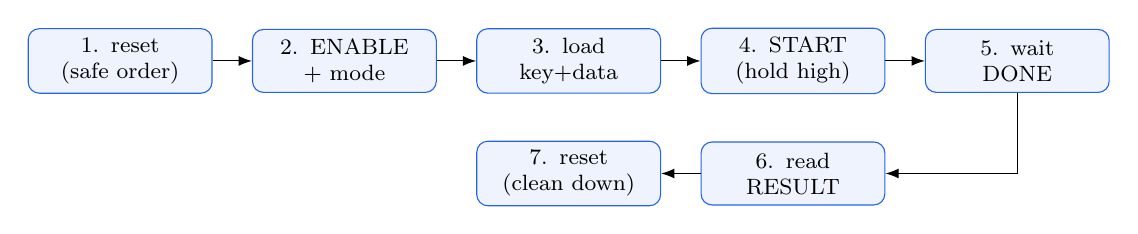
\begin{tikzpicture}[font=\footnotesize,node distance=3mm and 5mm,
  s/.style={draw=pblue,fill=pblue!8,rounded corners,minimum height=0.8cm,align=center,text width=2.1cm}]
  \node[s] (r) {1. reset\\(safe order)};
  \node[s,right=of r] (e) {2. ENABLE\\+ mode};
  \node[s,right=of e] (k) {3. load\\key+data};
  \node[s,right=of k] (st) {4. START\\(hold high)};
  \node[s,right=of st] (w) {5. wait\\DONE};
  \node[s,below=6mm of st] (rd) {6. read\\RESULT};
  \node[s,left=of rd] (cl) {7. reset\\(clean down)};
  \draw[-Latex](r)--(e);\draw[-Latex](e)--(k);\draw[-Latex](k)--(st);\draw[-Latex](st)--(w);
  \draw[-Latex](w.south)|-(rd);\draw[-Latex](rd)--(cl);
\end{tikzpicture}
\end{center}

\section{ASCON / Xoodyak offsets}
Identical maps (only the base differs). 128-bit KEY and NPUB are shifted in as
4$\times$32-bit writes; AD/PT go into FIFOs; CT/TAG are read back.
\begin{center}\rowcolors{2}{rowalt}{white}
\begin{tabular}{llp{7cm}}
\toprule
Offset & Register & Notes \\ \midrule
\code{0x00} & LEN & \code{\{triggercfg[23:16], pt\_len[15:8], ad\_len[7:0]\}} (byte lengths) \\
\code{0x04} & KEY & 32b $\times$4 $\rightarrow$ 128b \\
\code{0x08} & NPUB & 32b $\times$4 $\rightarrow$ 128b \\
\code{0x0C} & AD & write $\rightarrow$ AD FIFO \\
\code{0x10} & PT & write $\rightarrow$ PT FIFO \\
\code{0x14} & CT & read $\leftarrow$ CT FIFO \\
\code{0x18} & TAG & read $\leftarrow$ TAG FIFO \\
\bottomrule
\end{tabular}\end{center}

\begin{notebox}
\textbf{AEAD = hardware encrypt + software decrypt.} The ASCON and Xoodyak cores
implement the \emph{encryption} datapath --- the operation side-channel capture
measures --- and encrypt bit-exactly against the reference vectors. Decryption
and tag verification run on the host, so the workflow is: \textbf{encrypt on the
chip, decrypt + verify the tag on the PC} with \code{proact\_host/aead\_soft.py}
(bit-exact ASCON-128 v1.2 / Xoodyak v2; decrypt returns \code{None} on a wrong
tag; not constant-time --- for validation, not production keys). The firmware's
\code{decrypt=1} path is bounded, so a stray on-chip decrypt attempt returns
promptly rather than running. AES1/AES2 decrypt fully in hardware.
\end{notebox}

\subsection*{The \code{triggercfg} field --- selecting the trigger window}
For ASCON and Xoodyak the 7-bit \code{triggercfg} (LEN bits [23:16]) defines the
\emph{trigger window} = [start condition] $\rightarrow$ [stop condition], so that
exactly one phase of the operation can be captured.

\textbf{Step 1 --- mode} (\code{triggercfg[0]}):
\begin{itemize}[nosep,leftmargin=1.4em]
\item \textbf{Mode 0} (\code{triggercfg[0]=0}): the trigger goes LOW only when
\code{done\_o=1} --- simplest: start at the chosen state, stop at done.
\item \textbf{Mode 1} (\code{triggercfg[0]=1}): the trigger goes LOW at a
selected stop state (bits [6:4]).
\end{itemize}

\begin{center}\rowcolors{2}{rowalt}{white}
\begin{tabular}{cl@{\hskip 1.5cm}cl}
\toprule
\multicolumn{2}{c}{Activation \code{triggercfg[3:1]} (trigger HIGH at)} &
\multicolumn{2}{c}{Deactivation \code{triggercfg[6:4]} (Mode 1, LOW at)} \\ \midrule
0 & \code{S\_KEY} & 0 & \code{tr\_kEY\_n} \\
1 & \code{S\_NPUB} & 1 & \code{tr\_n\_s} \\
2 & \code{S\_AD} & 2 & \code{tr\_s\_p} \\
3 & \code{tr\_s\_p} & 3 & \code{S\_PT} \\
4 & \code{S\_PT} & 4 & \code{S\_IDLE} or \code{done\_o} \\
\bottomrule
\end{tabular}\end{center}
Example: \code{0x12} = Mode 0, rise at the nonce (\code{S\_NPUB}), fall on done ---
the verified default. Use \code{0x01} to capture the key-absorption phase only.
The \code{AEAD\_TRIG(mode,rise,fall)} macro / the GUI ``Internal trigger''
field build these values.

\section{PRNG (pseudo-random number generator)}
The RNG is a Linear-Feedback Shift Register (LFSR). The \textbf{controller}
enables/disables and reseeds it; the \textbf{Sw-RV target} core reads the
generated random values (the natural consumer). Software interface:
\begin{lstlisting}[style=c]
ctrl_set(CTRL_ENABLE_RNG); ctrl_flush();      // enable (or clear to disable)
proact_write32(0x80000000, 0x12345678);       // RNG seed register
// the Sw-RV target reads random words from its data-side RNG address
\end{lstlisting}

\section{Timer}
The timer is enabled/disabled by the controller and \textbf{counts clock cycles
while the trigger is high} --- so it measures the exact operation window. The
trigger is driven through the shared Status \& Control registers, which all cores
reach. Software interface:
\begin{lstlisting}[style=c]
ctrl_set(CTRL_ENABLE_TIMER); ctrl_flush();     // enable (or clear to disable)
uint32_t cycles = proact_read32(0x40000000);   // read the cycle count
\end{lstlisting}

% ================= CH7 C LIBRARY =================
\chapter{The Controller C Library}
Include \code{proact\_regs.h} (map) and the driver headers. Every function
encodes the safe access sequence for its peripheral.

\section{Device access + safe UART (\code{proact\_common.h})}
\begin{lstlisting}[style=c]
void     dev_write(uintptr_t addr, uint32_t val);   // 32-bit MMIO write
uint32_t dev_read (uintptr_t addr);                 // 32-bit MMIO read
int  putchar(int c);        // paced TX -- cannot overflow the 512B FIFO
int  puts(const char *str); // paced string TX
void put_hex(uint32_t h);   // 8-digit hex TX
int  uart_rx_ready(void);           // 1 if a byte is waiting (safe status read)
int  uart_getchar(void);            // BLOCK then read (never hangs on idle UART)
int  uart_getchar_timeout(uint32_t spins);
void uart_set_baud_divisor(uint32_t divisor);       // writes UART+0x04 only
void proact_idle_forever(void);     // park the core (NOT the old sim_halt!)
\end{lstlisting}

\section{Control + status registers}
\begin{lstlisting}[style=c]
// proact_ctrl.h -- shadow-register model; writes are absolute
void ctrl_reset(void);              // shadow = 0
void ctrl_set(uint32_t bits);       // shadow |= bits (use CTRL_* macros)
void ctrl_clr(uint32_t bits);       // shadow &= ~bits
void ctrl_flush(void);              // write shadow to hardware (bit31 masked)
void ctrl_flush_debug(int debug);
// proact_status.h -- status reads always answer, so waiting is safe
uint32_t status_read(void);
int  status_test(uint32_t mask);
void status_wait(uint32_t mask);                    // spin until mask set
int  status_wait_timeout(uint32_t mask, uint32_t spins);
\end{lstlisting}

\section{Crypto drivers}
\begin{lstlisting}[style=c]
// proact_aes.h    core = PROACT_AES1 | PROACT_AES2
void aes_run(proact_aes_core_t core, const uint32_t key[4],
             const uint32_t data[4], uint32_t out[4], uint32_t decrypt,
             uint32_t verbose);         // full safe reset->...->reset sequence
void aes_reset(proact_aes_core_t core);
// proact_aead.h   core = PROACT_ASCON | PROACT_XOODYAK
// NOTE: correct for ENCRYPT only -- hardware decrypt cannot complete (Ch.6);
// a decrypt attempt ends at the bounded status_wait_timeout and returns zeros.
void aead_run(proact_aead_core_t core, const uint32_t key[4],
              const uint32_t nonce[4], const uint32_t *ad, const uint32_t *pt,
              uint32_t *ct, uint32_t *tag, uint32_t ad_len, uint32_t pt_len,
              uint32_t decrypt, uint32_t triggercfg, uint32_t verbose);
// proact_aead_kat.h -- on-chip ASCON+Xoodyak encrypt known-answer test
int aead_kat_run(void);                    // reference vectors; CMD_AEADKAT 0x1A
// proact_experiments.h -- known-answer / round-trip self-tests
int run_all_experiments(uint32_t debug);   // returns number of FAILED suites
                                           // (AEAD decrypt half: expected FAIL)
\end{lstlisting}

\section{Sw-RV target driver (\code{proact\_swrv.h})}
\begin{lstlisting}[style=c]
void swrv_enable(void);              // release the target from reset (boots it)
void swrv_select_trigger(void);      // route the Sw-RV trigger to the scope
void swrv_load_imem_word(uint32_t off, uint32_t word);   // load target code
void swrv_load_dmem_word(uint32_t addr, uint32_t word);  // load target data
int  swrv_aes_block(const uint32_t key[4], const uint32_t in[4],
                    uint32_t out[4], int decrypt, uint32_t timeout);
\end{lstlisting}

% ================= CH8 TARGET =================
\chapter{The Target (Sw-RV) Software}
The target runs a portable AES-128 (encrypt + decrypt). The controller loads its
two images, releases it from reset, and exchanges data through the shared
data-memory mailbox --- \textbf{one command word and one done word per block},
not one handshake per data word (a significant speed-up over the previous flow).

\begin{center}
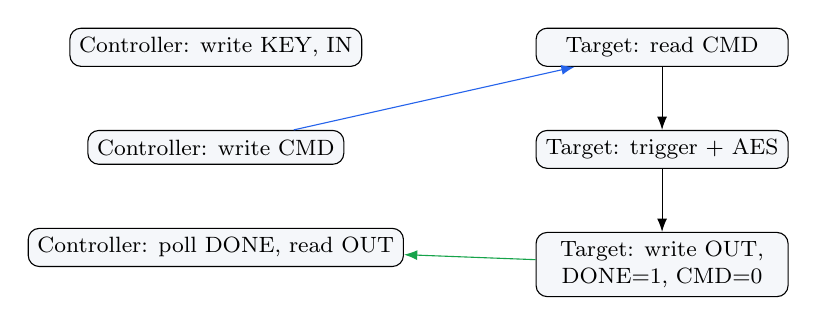
\begin{tikzpicture}[font=\footnotesize,node distance=8mm,
  b/.style={draw,rounded corners,fill=codebg,minimum width=3.2cm,align=center}]
  \node[b] (c1) {Controller: write KEY, IN};
  \node[b,below=of c1] (c2) {Controller: write CMD};
  \node[b,right=2.2cm of c1] (t1) {Target: read CMD};
  \node[b,below=of t1] (t2) {Target: trigger + AES};
  \node[b,below=of t2] (t3) {Target: write OUT,\\DONE=1, CMD=0};
  \node[b,below=of c2] (c3) {Controller: poll DONE, read OUT};
  \draw[-Latex,pblue] (c2) -- (t1);
  \draw[-Latex] (t1)--(t2); \draw[-Latex] (t2)--(t3);
  \draw[-Latex,tip] (t3) -- (c3);
\end{tikzpicture}
\end{center}
Mailbox addresses (shared, same on both sides): \code{KEY 0x08003F00},
\code{IN 0x08003F10}, \code{OUT 0x08003F40}, \code{CMD 0x08003F80},
\code{DONE 0x08003F84}. The Sw-RV cannot reach the UART, so it never prints; it
raises the scope trigger by writing status bit 31 (with \code{cfg\_sel}=Sw-RV).

% ================= CH9 BUILD/PROGRAM =================
\chapter{Building and Programming}
\section{Build outputs}
The \textbf{controller} build emits \emph{one} combined, absolute-addressed,
byte-swapped \code{main.vmem} (\code{.text} + \code{.data}/\code{.rodata} in a
single image --- the SPI loader routes each word by address), plus an
\code{.elf} and a disassembly. The \textbf{Sw-RV} build emits two images
(\code{sw\_rv\_imem.vmem} + \code{sw\_rv\_dmem.vmem}); its data (S-box tables)
lives in a loadable section --- confirmed present, not zeroed.

\section{The SPI code loader}
The MCP2210 streams 64-bit frames, \emph{address in the upper word}, MSB-first,
while driving the reset lines:
\begin{center}
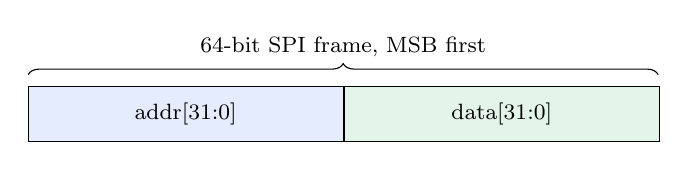
\begin{tikzpicture}[font=\footnotesize]
  \node[draw,fill=pblue!12,minimum width=4cm,minimum height=0.7cm] (a) at (0,0) {addr[31:0]};
  \node[draw,fill=tip!12,minimum width=4cm,minimum height=0.7cm,right=0 of a] (d) {data[31:0]};
  \draw[decorate,decoration={brace,amplitude=4pt}] (-2,0.5) -- (6,0.5) node[midway,above=3pt]{64-bit SPI frame, MSB first};
\end{tikzpicture}
\end{center}
Boot order: hold reset low $\rightarrow$ raise SPI reset $\rightarrow$ set
chip-select $\rightarrow$ stream $\rightarrow$ release reset to run. The GUI and
\code{proact program} perform this sequence automatically.

% ================= CH10 PYTHON =================
\chapter{The Python Host Library}
\code{import proact\_host}. Hardware backends are imported lazily, so the package
imports even without a bench attached.

\section{Transport --- \code{transport.py}}
\begin{lstlisting}[style=py]
from proact_host.transport import UartTransport, ProactTarget
t = UartTransport(port=None, baud=115200).open()   # None = auto-detect MCP2200
chip = ProactTarget(t)
chip.select("aes1"); chip.set_key(key16); chip.set_plaintext(pt16)
chip.set_decrypt(False); chip.enable_sendback()
mode, payload = chip.run_and_read()                # -> (mode, 16/32 bytes)
# other methods: set_nonce, set_ad, set_trigger_cfg(0x12), set_cfgsel("aes1"),
#                seed_rng, get_timer(), self_test(), load_target_imem/dmem,
#                read_status(), write_control(v), aead_kat() -> (xoo_ok, asc_ok)
\end{lstlisting}
For ASCON/Xoodyak, decryption runs on the host (the cores implement the
encryption datapath, Ch.~6). Decrypt on the PC instead:
\begin{lstlisting}[style=py]
from proact_host import aead_soft            # pure-Python, dependency-free
ct, tag = aead_soft.ascon128_encrypt(key, nonce, ad, pt)   # bit-exact vs chip
pt2 = aead_soft.ascon128_decrypt(key, nonce, ad, ct, tag)  # None on a bad tag
# same API for xoodyak_*; words_to_bytes/bytes_to_words convert chip words
\end{lstlisting}

\section{Programmer + resets}
\begin{lstlisting}[style=py]
from proact_host.programmer import Mcp2210Programmer
from proact_host.resets import ResetController
prog = Mcp2210Programmer().open()
prog.program("Software/Controller/main.vmem", progress=print)
rc = ResetController(prog)
rc.apply_mode("global")          # none|default_program|controller|global|spi
rc.status()                      # {line: True(active)/False(reset)/None}
\end{lstlisting}

\section{ChipWhisperer capture --- \code{capture.py}}
\begin{lstlisting}[style=py]
from proact_host.capture import ChipWhispererCapture
cap = ChipWhispererCapture(samples=5000, platform="asic")  # or "fpga" (CW305)
cap.connect(clock_hz=50e6)  # asic: Husky HS2 clkgen; fpga: CW305 PLL + extclk
cap.clock_status()  # {platform, target_clock_MHz, adc_freq_MHz, hs2,
                    #  clock_source, locked}
cap.arm(); # ... run the op ...; trace = cap.capture(); cap.disconnect()
\end{lstlisting}

\section{Experiment, storage, validation, inputs, self-check}
\begin{lstlisting}[style=py]
from proact_host.experiment import PROACTExperiment
with PROACTExperiment(platform="asic", target="aes1", traces=1000,
                      output="experiments/aes1") as exp:
    exp.prepare(); exp.capture(); exp.save()   # HDF5 (or NPZ) with metadata
# also: storage.TraceStore/load, validation.aes128_encrypt_block/validate_aes,
#       inputs.InputPlan/Variable/parse_input_file,
#       monitor.MonitorDecoder/safe_text (noise-tolerant UART decoding)
\end{lstlisting}
\textbf{The single unified live self-check} is
\code{proact\_host.fullcheck.run\_full\_check(target, scope=None, ...)} --- the
same engine behind the GUI's \textbf{Self-Check (A--Z)} tab. It sweeps the whole
system: UART link + baud, AES1/AES2 encrypt KAT + decrypt round-trip,
ASCON/Xoodyak on-chip encrypt KAT (\code{aead\_kat()}) + \code{aead\_soft}
software decrypt round-trip, timer, control write, PRNG, Sw-RV software AES, and
optional scope clock lock + trace capture. It \textbf{passes 100\% on the real
CW305 bench} and also serves as the ASIC chip-screening tool. (The older
\code{selfcheck.run\_self\_check} per-core check is superseded by it.)

% ================= CH11 CLI =================
\chapter{The Command-Line Interface}
\begin{center}\rowcolors{2}{rowalt}{white}
\begin{tabular}{p{5.5cm}p{8.5cm}}
\toprule
Command & Function \\ \midrule
\code{proact info} & print the address map + bench config \\
\code{proact devices} & list detected MCP2200/MCP2210 + ports \\
\code{proact build-controller} & build the controller firmware \\
\code{proact build-target} & build the Sw-RV firmware \\
\code{proact test} & host-side protocol + AES-reference self-check \\
\code{proact program --vmem main.vmem} & load firmware over MCP2210 SPI (full reset choreography) \\
\code{proact run --core aes1 ...} & run one operation, print the result \\
\code{proact capture --core aes1 --traces N} & capture a trace set \\
\code{proact selftest} & trigger the \emph{on-chip} self-test (\code{0x11}; its AEAD decrypt half runs on the host by design, Ch.~6) \\
\code{proact load-swrv} & load + start the Sw-RV software-AES target \\
\code{proact gui} & launch the GUI \\
\bottomrule
\end{tabular}\end{center}
Run the CLI through \code{./run\_cli.sh} (e.g.\ \code{./run\_cli.sh info}) so the
right Python is used --- never with \code{sudo}. The full A--Z \emph{live}
self-check is \code{fullcheck.run\_full\_check()} / the GUI's Self-Check
(A--Z) tab (Ch.~10).

% ================= CH12 GUI =================
\chapter{The Graphical User Interface}
Launch with \code{./run\_gui.sh} --- never with \code{sudo} (root breaks the
ChipWhisperer install; device access comes from the udev rules, Ch.~3). The
left sidebar is connection, reset control (with LED indicators) and programming:
connection and programming are always visible, while reset control is a
collapsible panel that starts \emph{collapsed} (click its header to expand it),
since it is a bring-up tool rather than a per-run control. The centre holds
\textbf{seven tabs}, one per workflow step, so no page has to be scrolled: the
crypto experiment, ChipWhisperer, \textbf{CPA analysis}, registers,
\textbf{Memory / Sw-RV}, \textbf{Self-Check (A--Z)} and the UART monitor. Every
panel has a \textbf{(?)} help button.

\begin{center}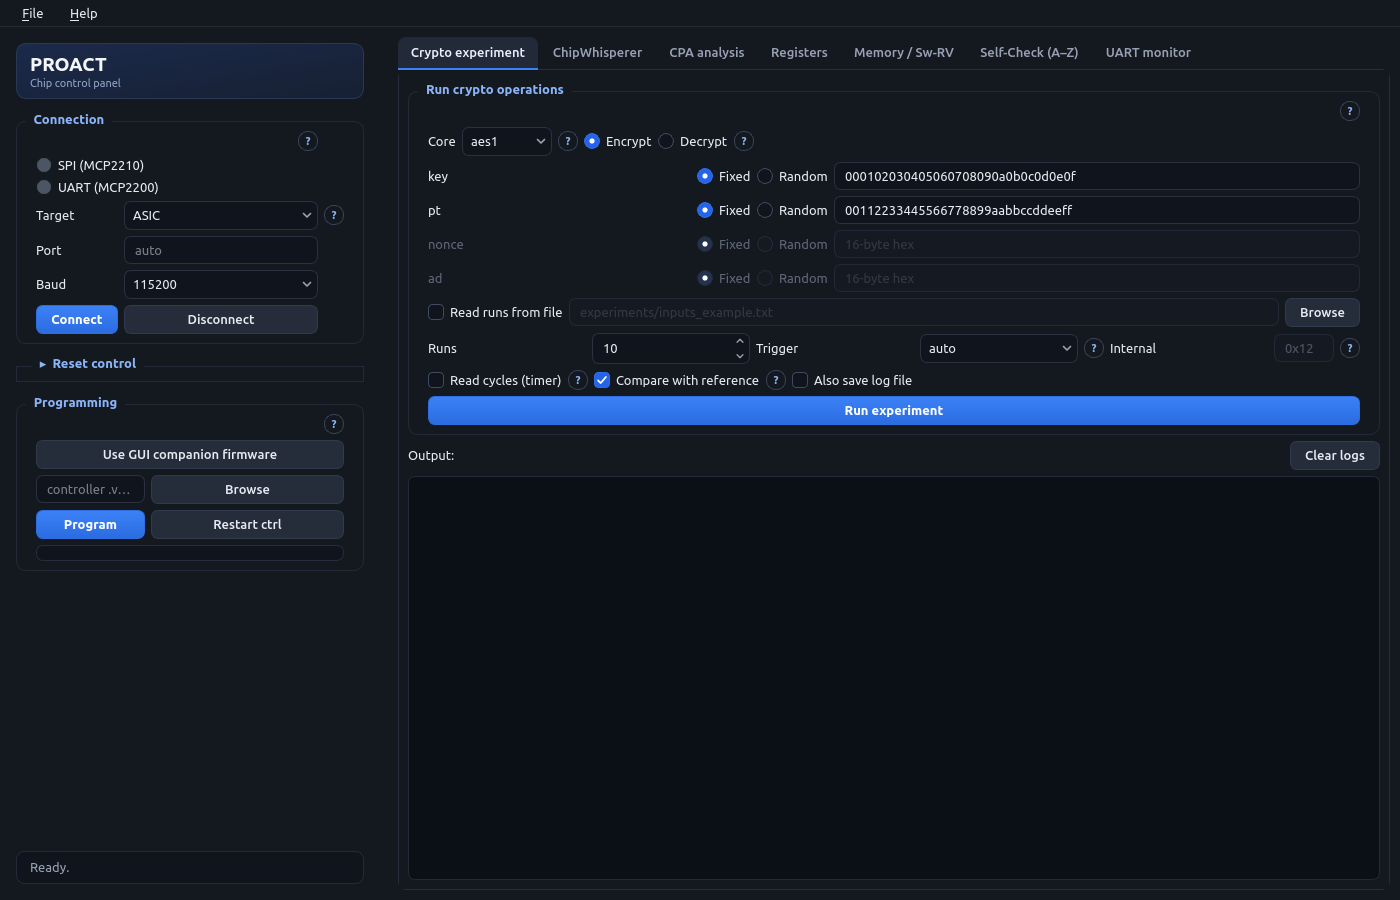
\includegraphics[width=\textwidth]{gui_overview.png}\end{center}
\textbf{Crypto experiment:} pick a core (nonce/AD auto-disable for AES), choose
encrypt/decrypt, set each input Fixed or Random (or read a whole run list from a
text file), set the number of runs, the trigger source and the internal
(ASCON/Xoodyak) trigger phase, optionally read the cycle count, and compare each
result with a software reference. Output goes to the window and optionally a log.
For ASCON/Xoodyak, decryption runs on the host with \code{aead\_soft}
(Ch.~6) --- the cores implement the encryption datapath --- so
a \emph{Decrypt} attempt there ends at the firmware's bounded timeout and
returns zeros. AES1/AES2 decrypt normally.

\begin{center}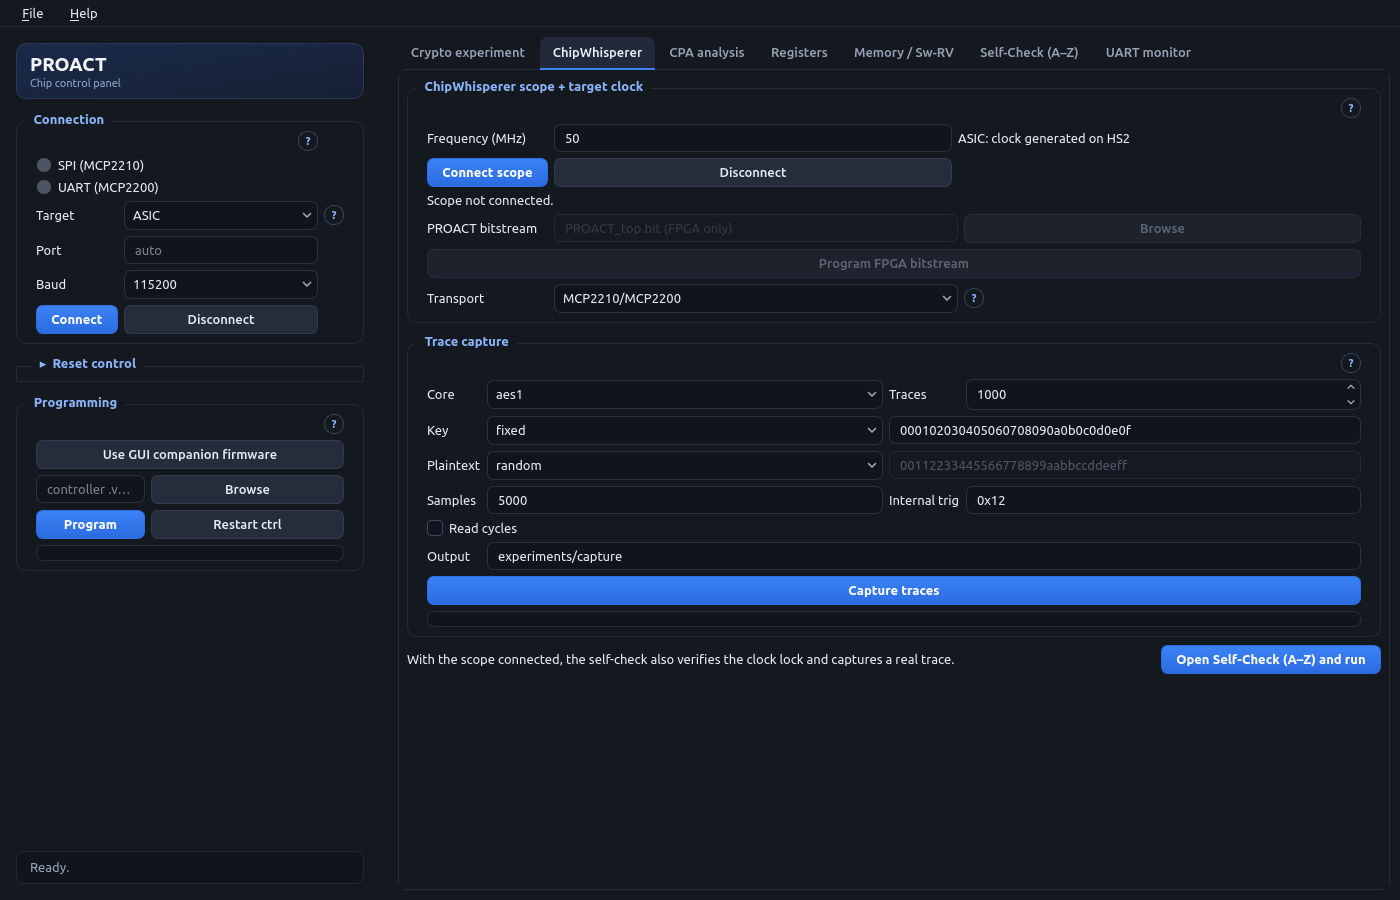
\includegraphics[width=\textwidth]{gui_chipwhisperer.png}\end{center}
\textbf{ChipWhisperer:} connect/disconnect the Husky, set the target clock
(ASIC: 50\,MHz on HS2; FPGA: program the CW305 bitstream, on-board PLL), choose
the transport (MCP bridges or the Husky's own SPI/UART with GPIO3 chip-select),
and capture traces. There is no separate self-check panel here: one compact row
at the bottom of the page --- a one-line reminder plus the single button
\emph{Open Self-Check (A--Z) and run} --- jumps to the Self-Check tab and runs it.

\begin{center}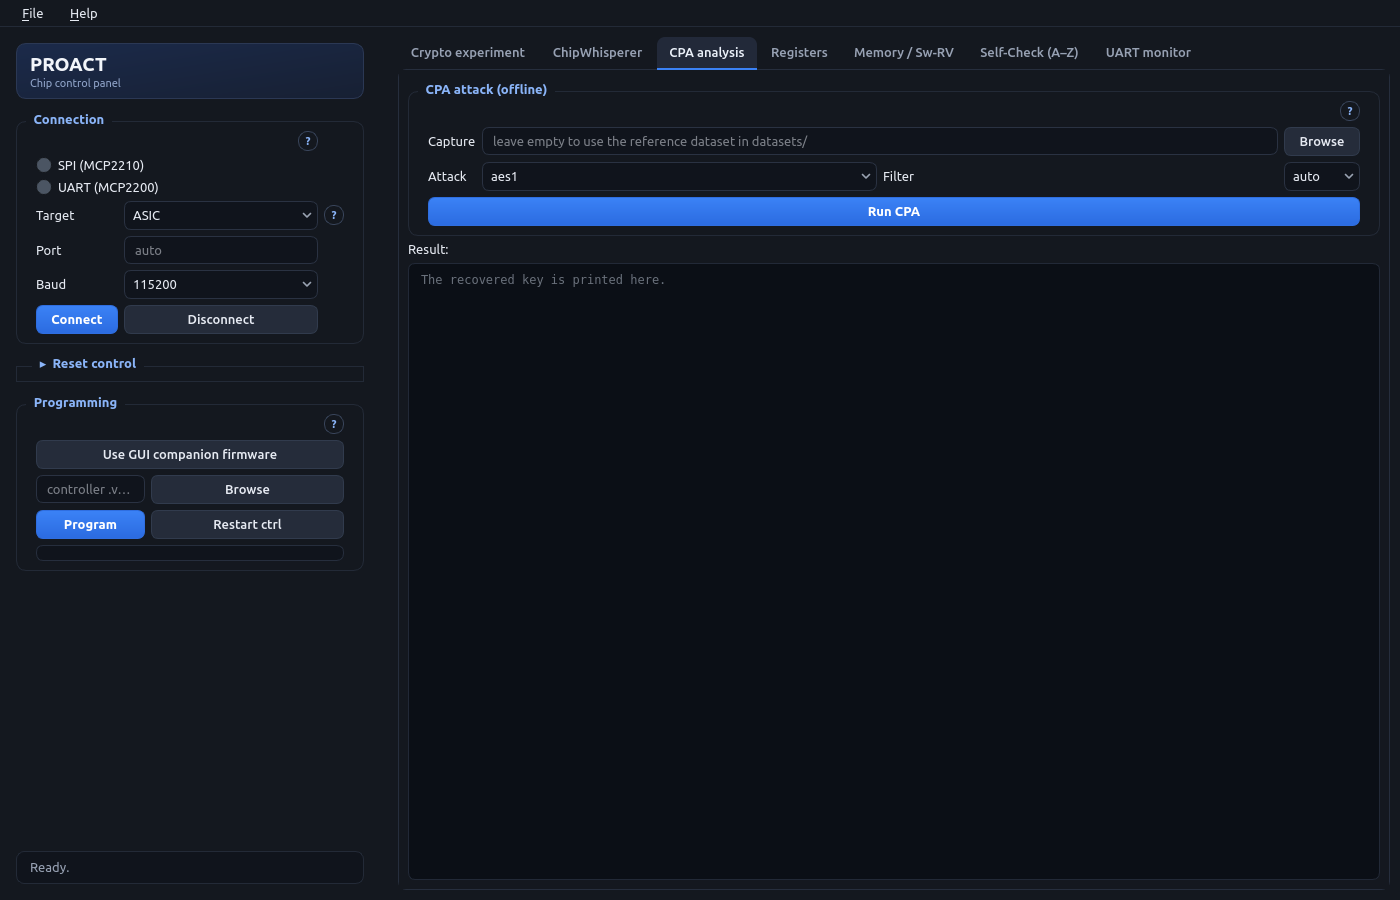
\includegraphics[width=\textwidth]{gui_cpa.png}\end{center}
\textbf{CPA analysis:} the offline correlation power-analysis attack, on its own
page. Leave \emph{Capture} empty to attack the reference traces shipped in
\code{datasets/}, or browse to your own \code{.npz}/\code{.h5}; pick the leakage
model (\code{aes1}/\code{aes2} last-round ciphertext, \code{swrv} first-round
S-box) and the moving-average filter width (\emph{auto} picks it from the data;
measured best AES1 8, AES2 2, Sw-RV 16), then \emph{Run CPA}. It needs no
hardware, so it doubles as a no-board demo; the recovered key is printed in the
console that fills the rest of the page.

\begin{center}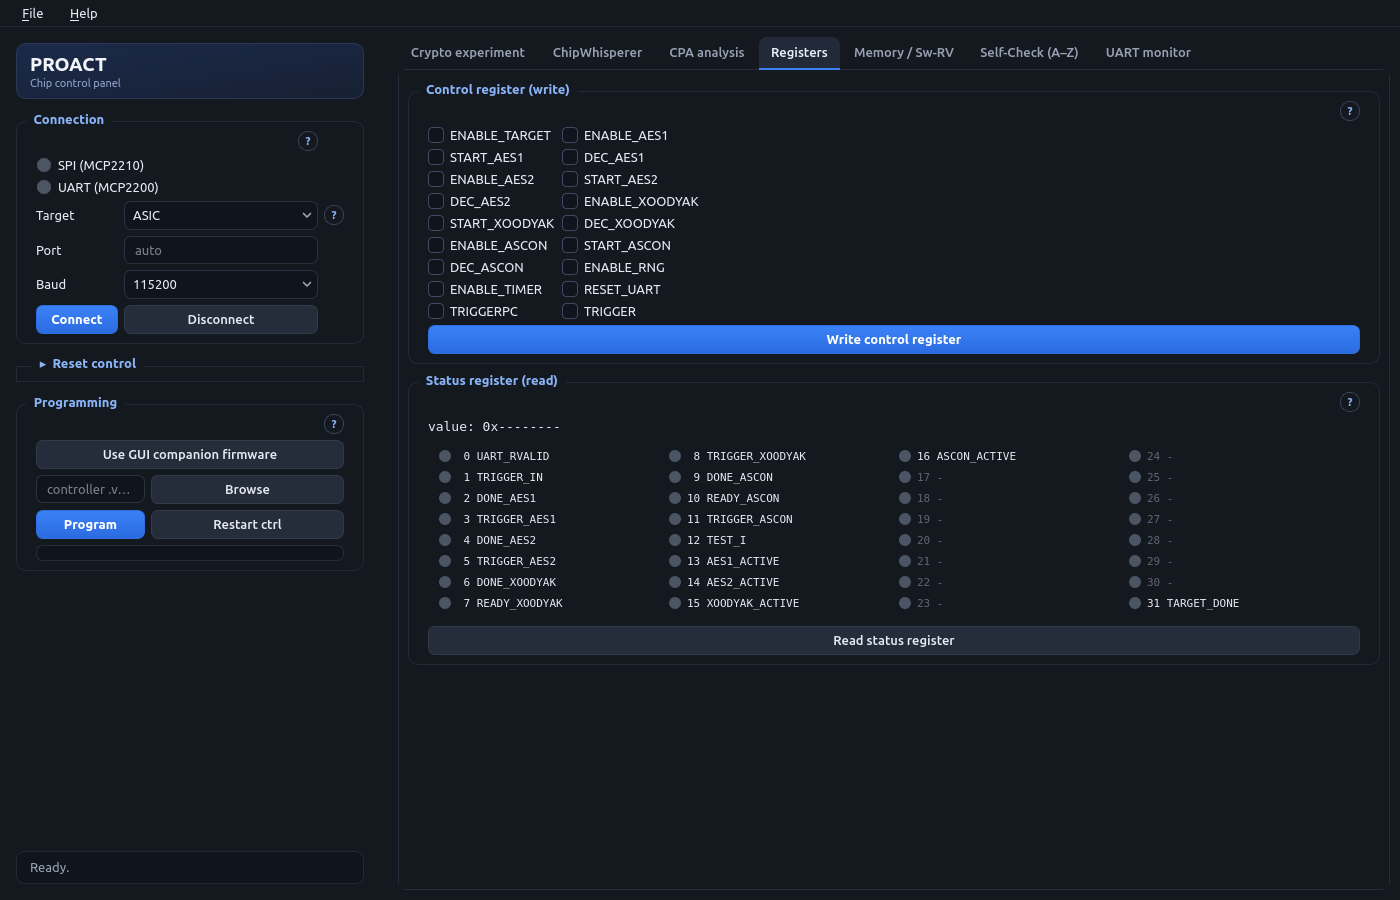
\includegraphics[width=\textwidth]{gui_registers.png}\end{center}
\textbf{Registers:} tick control-register bits and write them; read the status
register and see each set bit light up with its meaning in a grid of 8 rows by
4 columns.

\begin{center}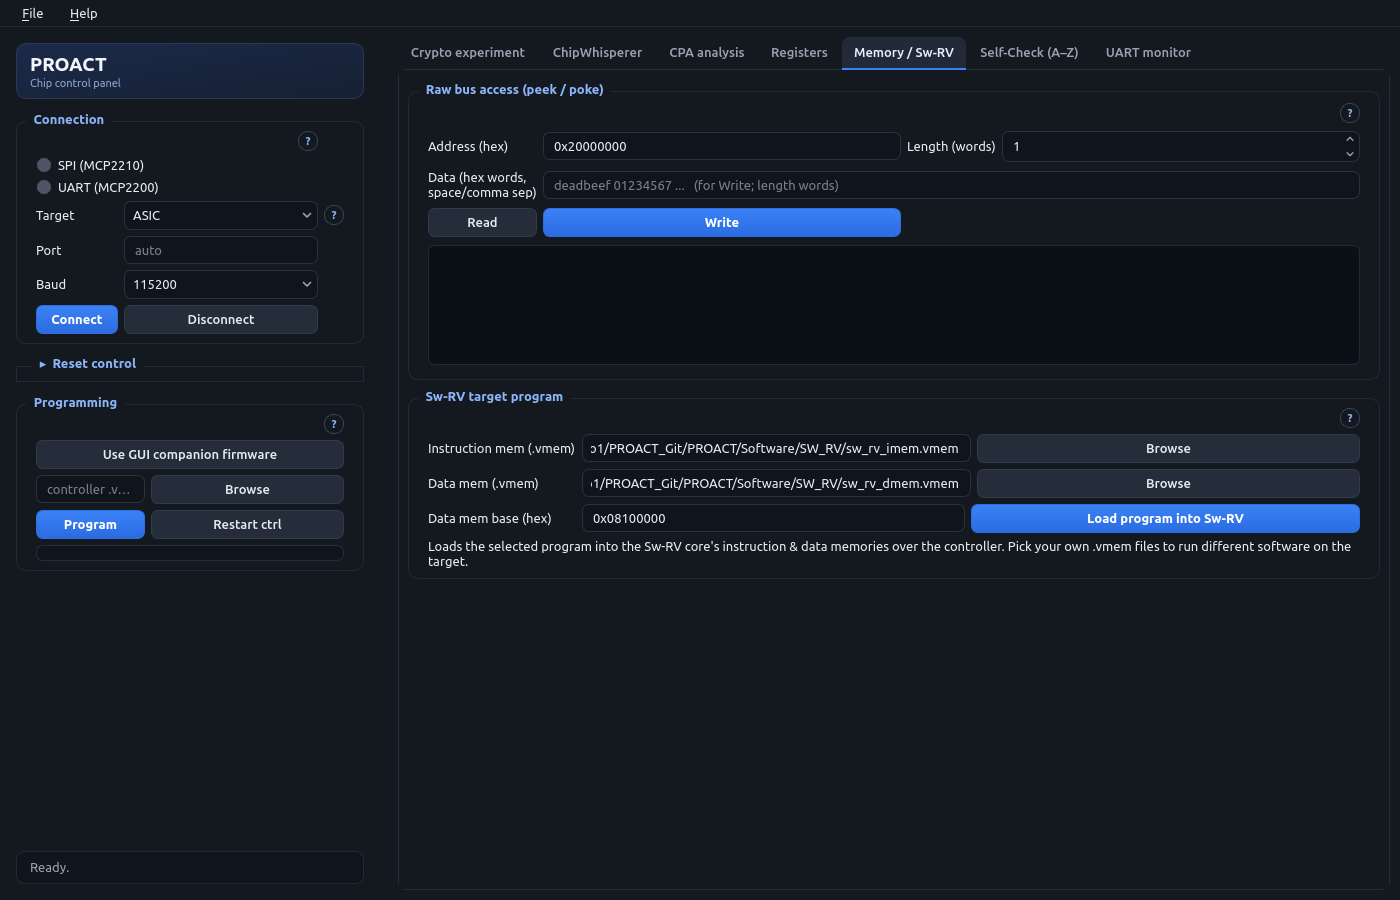
\includegraphics[width=\textwidth]{gui_memory.png}\end{center}
\textbf{Memory / Sw-RV:} the two bring-up and debug panels. \emph{Raw bus
access} peeks and pokes any bus address directly through the controller (32-bit
words, stepping 4 bytes) --- reads are safe on mapped addresses, but writing to
CPU RAM can wedge the chip, so poke only known addresses. \emph{Sw-RV target
program} loads the instruction and data \code{.vmem} images (defaults in
\code{Software/SW\_RV/}) at the data-mem base \code{0x08100000} while the target
is held in reset, then releases it so the fresh program boots; afterwards select
core \code{swrv} in the crypto experiment tab to run it.

\begin{center}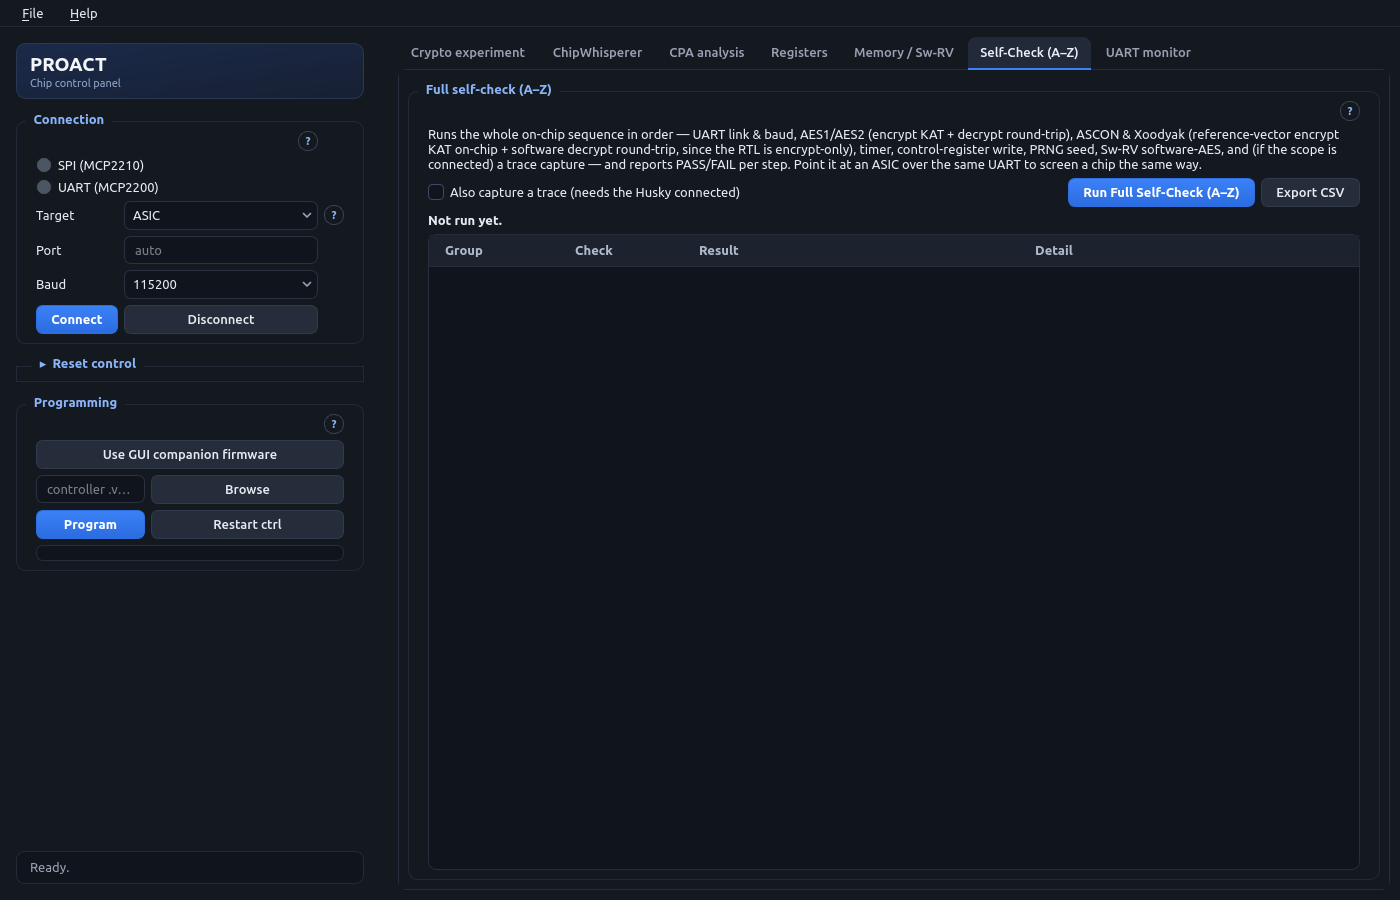
\includegraphics[width=\textwidth]{gui_selfcheck.png}\end{center}
\textbf{Self-Check (A--Z):} the single unified live check
(\code{fullcheck.run\_full\_check}, Ch.~10) with a live PASS/FAIL/SKIP table and
CSV export --- passes 100\% on the real CW305; also the ASIC screening tool.

% ================= CH13 CHIPWHISPERER =================
\chapter{ChipWhisperer and Trace Capture}
\section{Choosing the target: ASIC or FPGA}
The same PROACT design and the same UART/SPI software run on two platforms, but
the \textbf{clock} and \textbf{programming} differ --- pick the target in the
GUI's Connection panel (or set \code{platform} in \code{ChipWhispererCapture}):
\begin{center}\rowcolors{2}{rowalt}{white}
\begin{tabular}{p{2cm}p{6cm}p{5.5cm}}
\toprule
Platform & Clock & Program \\ \midrule
\textbf{ASIC} & the Husky generates the target clock on HS2 (\code{clkgen}, default 50\,MHz) & load the controller firmware \code{.vmem} over MCP2210 SPI \\
\textbf{FPGA (CW305)} & HS2 disabled; the CW305's on-board PLL provides the clock (output 1, 50\,MHz) & first upload the PROACT bitstream (\code{cw.target(scope, cw.targets.CW305, bsfile=…, fpga\_id="100t")}, VCCINT 1.0\,V), then load the firmware \\
\bottomrule
\end{tabular}\end{center}
The GUI's ChipWhisperer tab exposes the frequency (ASIC) and the bitstream +
``Program FPGA bitstream'' button (FPGA). The \textbf{GUI companion firmware} ---
the controller command server (\code{Software/Controller/main.vmem}) --- is
the on-chip program that understands all the GUI's commands; the Programming panel
has a one-click button to select it.

The capture order matches the verified PROACT trigger sequence:
\begin{center}
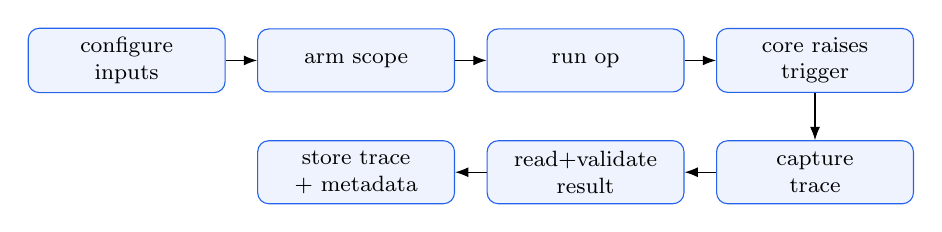
\begin{tikzpicture}[font=\footnotesize,node distance=4mm,
  s/.style={draw=pblue,fill=pblue!8,rounded corners,minimum width=2.5cm,minimum height=0.8cm,align=center}]
  \node[s](i){configure\\inputs};
  \node[s,right=of i](ar){arm scope};
  \node[s,right=of ar](ru){run op};
  \node[s,right=of ru](tr){core raises\\trigger};
  \node[s,below=6mm of tr](ca){capture\\trace};
  \node[s,left=of ca](re){read+validate\\result};
  \node[s,left=of re](sv){store trace\\+ metadata};
  \draw[-Latex](i)--(ar);\draw[-Latex](ar)--(ru);\draw[-Latex](ru)--(tr);
  \draw[-Latex](tr.south)--(ca);\draw[-Latex](ca)--(re);\draw[-Latex](re)--(sv);
\end{tikzpicture}
\end{center}
Set the target clock on HS2 (default 50\,MHz), select the trigger source to match
the core being captured (the firmware auto-sets \code{cfg\_sel}), arm, run, and
the scope captures the trigger window. Traces plus full metadata (key, plaintext,
output, scope + trigger settings, timestamp) are saved incrementally so a long
run survives interruption.

% ================= CH14 EXPERIMENTS =================
\chapter{Experiments and Data Storage}
Datasets are stored in HDF5 (rich, one file) or NumPy \code{.npz} (fallback).
Each stores traces, plaintexts, keys, outputs, validation flags, a failed-capture
log, and metadata (target, platform, scope/trigger settings, timestamp,
configuration). Input files (\code{experiments/inputs\_example.txt}) list one run
per line as \code{key=.. pt=.. nonce=.. ad=..} (hex).

% ================= CH15 TESTING =================
\chapter{Testing and Verification Status}
\begin{notebox}
The FPGA build is now \textbf{bench-verified end to end}: on a real CW305 +
Husky the unified A--Z self-check passes 100\% (16 pass, 0 fail, 0 skip;
2026-08-07). The fabricated \textbf{ASIC has not been screened yet} --- the same
A--Z check is the screening tool. Every claim below states exactly how it was
verified.
\end{notebox}
\begin{center}\rowcolors{2}{rowalt}{white}
\begin{longtable}{p{6.6cm}p{7.4cm}}
\toprule
Layer & Status \\ \midrule\endhead
\code{proact\_regs.h} vs frozen RTL & \textbf{RTL cross-checked} --- 34/34 constants agree \\
AES driver register sequence & \textbf{RTL-simulated} --- reproduces the known-answer ciphertext against the real \code{aes\_core} (iverilog) \\
Controller + target firmware & \textbf{builds clean} (0 warnings); one combined controller vmem, two Sw-RV vmem images \\
Host protocol + AES reference & \textbf{unit-tested} (byte-stream + FIPS-197 vector) \\
GUI & \textbf{constructs + renders} headless \\
On-chip AEAD encrypt KAT & \textbf{hardware} --- ASCON + Xoodyak both PASS on the CW305 (\code{CMD\_AEADKAT}) \\
On real FPGA (CW305 + Husky) & \textbf{hardware} --- full A--Z self-check passes 100\%, incl.\ scope lock + trace capture \\
AEAD decrypt & \textbf{runs on the host by design} --- \code{aead\_soft}, bit-exact round trip (Ch.~6) \\
On the fabricated ASIC & \textbf{not yet run} --- screened with the same A--Z check \\
\bottomrule
\end{longtable}\end{center}
Run all offline checks: \code{RTL\_ROOT=/path/to/ASIC/rtl bash tools/verify\_all.sh}.
Run the live A--Z check: the GUI \textbf{Self-Check (A--Z)} tab or
\code{proact\_host.fullcheck.run\_full\_check()}.

% ================= CH16 TROUBLESHOOTING =================
\chapter{Troubleshooting}
\begin{center}\rowcolors{2}{rowalt}{white}
\begin{longtable}{p{4.6cm}p{4.6cm}p{4.4cm}}
\toprule
Symptom & Likely cause & Fix \\ \midrule\endhead
CPU waits on an access & accessed a disabled core / reserved \code{Co\_re} slot / read UART before a byte arrived & use the library sequences (Ch.2); they wait on the right ready bit \\
Output stops mid-print & TX FIFO filled faster than the line drains (not a real freeze) & keep \code{putchar} pacing; scale it if the baud rate is lowered \\
No MCP device found & udev rules / wrong serial & install rules (Ch.3); set serials in \code{config.py} \\
Wrong/garbled UART text & wrong baud vs input clock & set the clock in \code{config.py} \\
Trigger never fires & wrong \code{cfg\_sel} (source) for the running core & use \code{CTRL\_TRIGGER}=bit30; select the trigger source; Sw-RV uses status bit 31 \\
Build error & toolchain not found & pass \code{RISCV=} to make (Ch.3) \\
On-chip AEAD decrypt returns all zeros & by design --- AEAD decrypt runs on the host (cores implement the encryption datapath, Ch.6) & decrypt + tag-verify on the PC: \code{proact\_host/aead\_soft.py} \\
Tools fail to start / modules missing / ``chipwhisperer is not installed'' & bare \code{python3} is the wrong interpreter (pyenv), or running as \code{sudo} & always launch \code{./run\_gui.sh} / \code{./run\_cli.sh}; never \code{sudo} --- udev rules give device access (Ch.3) \\
\bottomrule
\end{longtable}\end{center}

\appendix
\chapter{Chip Pinout}
The fabricated PROACT chip has 28 pins (package view: top, notch up). Reset lines
are active-low; the \code{out\_pins[*]} are debug/test outputs (several double as
trigger/status probes). Two useful bring-up details from the package:
\begin{itemize}[nosep,leftmargin=1.4em]
\item \textbf{The reset inputs have internal pull-ups} (\code{B\_RST\_N},
\code{spi\_global\_RST\_N}, \code{C\_RST\_N}, \code{spi\_c\_RST\_N} --- ``IN\,$\cdot$\,PU'')
enabled on silicon, so they idle at 3.3\,V (de-asserted) when left open.
\item \textbf{Four pins were reassigned to power during packaging} vs the RTL pad
list: pins 15 and 28 are \code{VDD} 0.8\,V core, pin 22 is \code{VDDIO} 3.3\,V,
and pin 20 is \code{spi\_c\_RST\_N} --- the table below is the \emph{as-packaged}
assignment (the wiring reference for the bench). The hardware design team's
package drawing can be placed at \code{docs/images/pinout.png}.
\end{itemize}
\begin{center}\rowcolors{2}{rowalt}{white}
\begin{longtable}{clllp{5.3cm}}
\toprule
\# & Name & Dir & Category & Description \\ \midrule\endhead
1 & \code{B\_RST\_N} & In·PU & Reset & board/push-button global reset (active-low) \\
2 & \code{TX} & Out & UART & UART transmit \\
3 & \code{RX} & In & UART & UART receive \\
4 & \code{spi\_global\_RST\_N} & In·PU & Reset & SPI global reset (active-low) \\
5 & \code{C\_RST\_N} & In·PU & Reset & controller reset (active-low) \\
6 & \code{out\_pins[0]} & Out & Debug & \code{data\_addr\_spi[23]} (SPI mem select) \\
7 & \code{VDDIO} & Pwr & Power & 3.3\,V I/O supply \\
8 & \code{VSS} & Pwr & Power & ground \\
9 & \code{SYSCLK\_P} & In & Clock & main system clock input \\
10 & \code{spare\_io} & In & Debug/Status & mapped to \code{status\_reg[1]} \\
11 & \code{out\_pins[5]} & Out & Debug/Status & \code{status\_bus.uart\_rvalid} \\
12 & \code{out\_pins[6]} & Out & Debug & \code{dev1\_req[RII\_data/in\_mem]} \\
13 & \code{out\_pins[1]} & Out & Debug/Trigger & \code{trigger\_cfg} \\
14 & \code{trigger\_Out} & Out & Trigger & \textbf{global trigger output} \\
15 & \code{Vcore} & Pwr & Power & core supply (0.8\,V) \\
16 & \code{out\_pins[7]} & Out & Debug & \code{flash\_dout} (heartbeat LED) \\
17 & \code{SIn} & In & SPI & SPI serial data in (MOSI) \\
18 & \code{SSel\_n} & In & SPI & SPI chip select (active-low) \\
19 & \code{sck} & In & SPI & SPI serial clock \\
20 & \code{spi\_c\_RST\_N} & In·PU & Reset & SPI controller reset (active-low) \\
21 & \code{out\_pins[11]} & Out & Debug & AES1/AES2/Xoodyak/ASCON request \\
22 & \code{VDDIO} & Pwr & Power & 3.3\,V I/O supply \\
23 & \code{trigger\_in} & In & Trigger & external trigger input \\
24 & \code{out\_pins[4]} & Out & Debug & \code{SW\_RV pc\_out[4]} \\
25 & \code{out\_pins[3]} & Out & Debug & \code{SW\_RV pc\_out[3]} \\
26 & \code{out\_pins[2]} & Out & Debug & \code{SW\_RV pc\_out[2]} \\
27 & \code{out\_pins[8]} & Out & Debug/Trigger & \code{trigger\_reserve} (Ctrl-RV trigger) \\
28 & \code{Vcore} & Pwr & Power & core supply (0.8\,V) \\
\bottomrule
\end{longtable}\end{center}

\chapter{Quick Reference}
\section{UART command bytes}
\code{0x01} KEY $\cdot$ \code{0x02} PT $\cdot$ \code{0x03} send-back $\cdot$
\code{0x04} debug $\cdot$ \code{0x05} run $\cdot$ \code{0x06} AES2 $\cdot$
\code{0x07} Xoodyak $\cdot$ \code{0x08} ASCON $\cdot$ \code{0x09} AES1 $\cdot$
\code{0x0A} arm $\cdot$ \code{0x0B} NONCE $\cdot$ \code{0x0C} AD $\cdot$
\code{0x0D} dec $\cdot$ \code{0x0E} seed $\cdot$ \code{0x0F} trig-cfg $\cdot$
\code{0x10} timer $\cdot$ \code{0x11} self-test $\cdot$ \code{0x12} load-imem $\cdot$
\code{0x13} load-dmem $\cdot$ \code{0x14} Sw-RV $\cdot$ \code{0x15} cfg-sel $\cdot$
\code{0x16} read-status $\cdot$ \code{0x17} write-ctrl $\cdot$ \code{0x18} poke $\cdot$
\code{0x19} peek $\cdot$ \code{0x1A} AEAD KAT.
Result frame: \code{0xA5 <mode> <len> <payload>}.

\section{Summary of rules}
Trigger = bit 30. Enable a core before access. One core at a time. Leave the
reserved \code{0x10007000} slot alone. Read the UART when RX is ready.
ASCON/Xoodyak decrypt on the host (\code{aead\_soft}). Launch via
\code{./run\_gui.sh} / \code{./run\_cli.sh} --- never \code{sudo}. Edit
\code{hardware.json}, not the generated files.

\end{document}
